% Capítulo 4
\chapter{Taxonomia}
\label{cap:cap4}

Prosseguindo a análise dos trabalhos mencionados no Capítulo \ref{cap:cap3}, verifica-se a necessidade de classificar dos conceitos mais recorrentes atrelados ao uso do padrão \textit{throttling} em especial aos dispositivos em computação dirigida à energia. Além disso, é preciso levar em consideração a orientação do trabalho junto aos critérios de dependabilidade, em especialmente ao concentrar sobre o atributo disponibilidade, elemento participante nos critérios de dependabilidade apresentados na taxonomia proposta por \citeauthor{avizienis_basic_2004} (\citeyear{avizienis_basic_2004}). Por definição temos que disponibilidade é um indicador da capacidade de um equipamento, sistema ou serviço estar em um estado que possa desempenhar certa função solicitada quando necessário \cite{ISO9000}. 


\section{Organização}

As classes descritas foram categorizadas para acomodar os elementos envolvidos de acordo com os critérios que representam. À esquerda, apresenta-se as características dos dispositivos \acs{IoT} encontrados em cenários de restrições energéticas. Primeiramente, as classes foram projetadas para organizar os elementos em destaque considerando as especificidades e limitações à operar em ambientes com recursos energéticos limitados. Estes critérios, auxiliam na compreensão mais precisa em relação as categorias e podem ser visualizados na divisão básica dos elementos presentes na taxonomia, Figura \ref{fig:cap4divisaobasetaxonomia}. 

%agentes
Enquanto ao fator que caracteriza um agente, o destacado trabalho de \citeauthor{avizienis_basic_2004} (\citeyear{avizienis_basic_2004}) aplica a dinâmica de definição por papéis, proporciona clara divisão entre agentes em referencia ao que desempenha em relação ao ambiente inserido. Sendo assim, são propostos dois grupos: clientes, que atua ativamente realizando solicitações ou de forma passiva solicitando recursos ou quando notificado; e um segundo grupo, provedores, para estes cabe a responsabilidade de compartilhar seus recursos com outros consumidores através de uma interface conhecida de acordo com o protocolo pré-estabelecido entre as partes.

%Operaçoes
Toda interação segue um padrão denominado operação, esta é realizada de acordo com o qual se destina, como visto no trabalho de \cite{khairnar_discrete-rate_2015} operações podem ser medidas pela quantidade de mensagens trocadas entre dispositivos contribuindo para um determinado fim. Sendo assim, os elementos classificadores foram: \textit{Agentes}, \textit{Recursos} e \textit{Operações}.

%recursos
Percebeu-se a necessidade de classificar as características energéticas dos elementos participantes, ao passo que agentes fazem uso de um fator energético para realizar suas capacidades, colocando esses recursos energéticos como classe fundamental de analise, impulsionada pelos fatores gerais dos elementos ligados à \acs{IoT}, especialmente aderente aos conceitos de sistemas com  capacidade de coleta energética (\aclp{EHS}) relacionados com computação dirigida à energia.


\begin{figure}[hbt]
	\centering
	\caption{Divisão Base da Taxonomia}
	\label{fig:cap4divisaobasetaxonomia}
	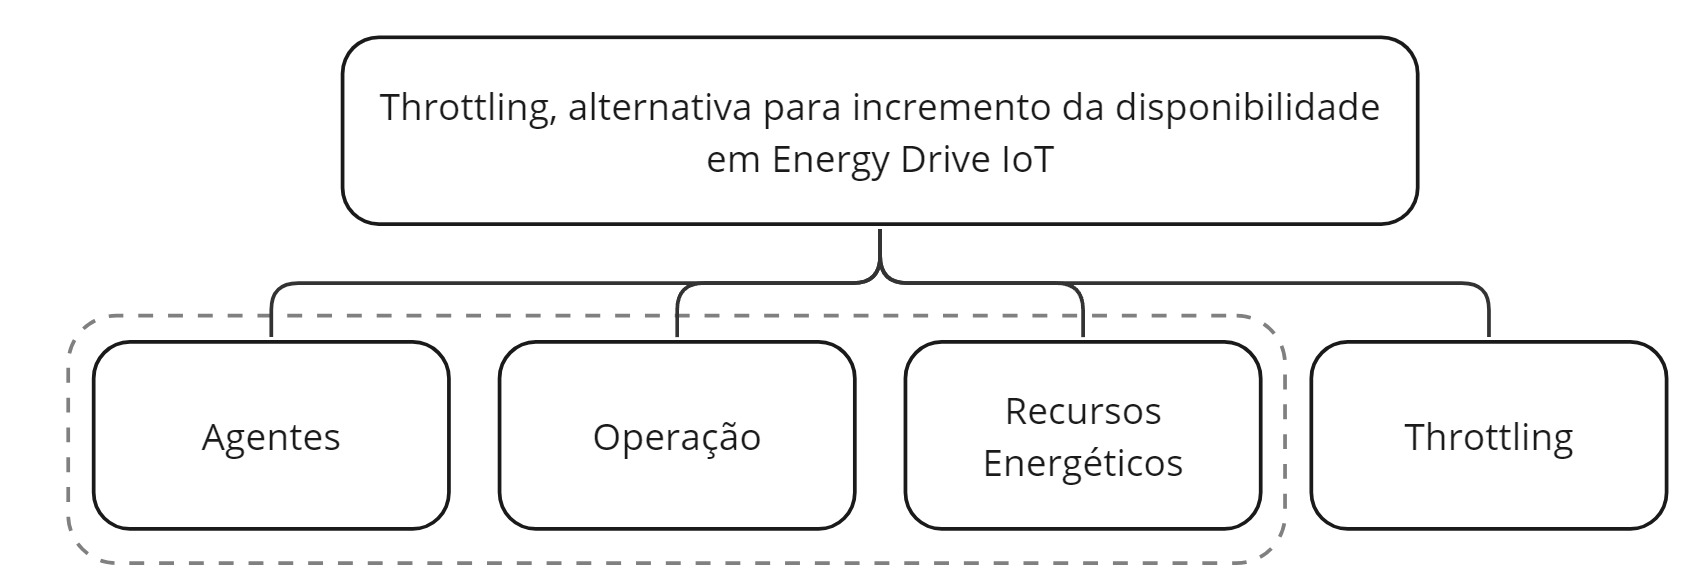
\includegraphics[width=0.7\linewidth]{Imagens/cap4/cap4taxonomia_primeironivel.jpg}	
	
	Fonte: elaborado pelo autor.
\end{figure}

Ademais, acomoda-se os elementos envolvidos no processo de gestão do comportamento de um dispositivo através do padrão \textit{Throttling}. Nesta classe, dois ramos principais são derivados, Atuação e Motivadores respectivamente. Sobre a classe Atuação, agrupa-se os elementos envolvidos no processo de ajuste de comportamento do: Limiar (\textit{Thresholding}), Ciclos, Meios e Observáveis. Finalmente, a classe Motivação é sugerida de maneira à assegurar as intenções enquanto busca incremento de disponibilidade. 

\begin{figure}[hbt]
	\centering
	\caption{Visão Geral da Taxonomia.}
	\label{fig:visaogeraltaxonomia}
	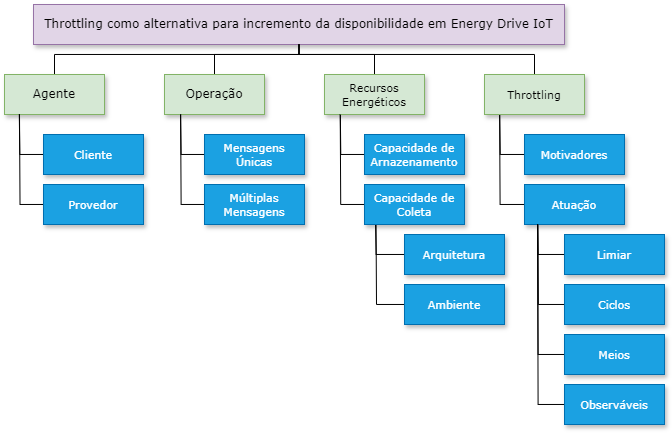
\includegraphics[width=\textwidth]{Imagens/anexos/anexo_visaogeraltaxonomia.png}	
	
	Fonte: elaborado pelo autor.
\end{figure}

\section{Taxonomia Proposta}
A Figura \ref{fig:visaogeraltaxonomia} ilustra a taxonomia visualmente com os pontos abordados no processo de escolha do padrão \textit{throttling} como alternativa para garantir disponibilidade nos agentes \acs{IoT} presentes em um ambiente. O objetivo principal é dispor os elementos ligados ao tema de maneira visual e contemplar a organização dos tópicos envolvidos. Com isso, compreende os objetivos almejados ao criar a taxonomia:

\begin{enumerate}
    \item Auxiliar a compreensão dos conceitos relacionados aos agentes \acs{IoT} em computação dirigida à energia e os tópicos inerentes à possibilidade de uso do padrão \textit{throttling} como elemento colaborador à disponibilidade desses agentes. Acomodadas em função de cada contexto e necessidade;
  	\item Oferecer suporte às definições de uso do padrão \textit{Throttling} ligados ao contexto \acs{IoT} dirigida a energia. 
  	\item Facilitar a descoberta das relações entre os elementos do campo de análise.
\end{enumerate}

\section{Agentes \acs{IoT}}
Cada agente é essencialmente uma entidade que tem a capacidade intrínseca de interagir com outros agentes sejam digitais ou agentes físicos, chamados dispositivos. Eles possuem propriedades fundamentais, como funcionalidade, desempenho e segurança \cite{avizienis_basic_2004}. No contexto da Internet das Coisas, é crucial considerar a capacidade de se comunicar com outras entidades, atuando em conjunto mediante compartilhamento de recursos, características intrínsecas nos dispositivos \acs{IoT} \cite{asghari_internet_2019}.


\subsection{Dispositivo Provedor}

Em qualquer instância onde um dispositivo oferece estados ou atende solicitações de recurso, assume o papel de provedor. Para isso, o dispositivo oferece uma ou mais funcionalidades denominadas operações, sendo cada uma, realizada através do uso de seus recursos a medida que avança em seus estados internos buscando fornecer resposta as solicitações. O resultado disto será percebido como estado externo, acessível por meio de sua interface em resposta às solicitações ou provida na forma de eventos acessíveis aos clientes. 

A medida que solicitações se apresentam ao dispositivo provedor, tais eventos interagem na forma como este lida com seus recursos. Através disso, motivam a dinâmica de mudanças de estado internos e por sua vez impactam diretamente na dinâmica dos custos operacionais do dispositivo.  Por exemplo, tomemos um sistema de iluminação urbana que pode, por meio de solicitações, interagir com dispositivos encontrados em um ambiente. Assim, este sistema atua solicitando aos dispositivos a mudança de estado para que acione um recurso em razão de um evento qualquer. Tal ação impactará no uso  dos componentes necessários em decorrência do atendimento das solicitações e assim, impactando na forma como o provedor utiliza seus recursos.


\subsection{Dispositivo Cliente}
Um dispositivo cliente é um agente físico que realiza o papel responsável por receber o estado externo de dispositivos provedores por meio de uma interface de interação disponibilizada. Ele pode consumir recursos provenientes de um ou mais provedores, dependendo da operação que precisa realizar. De forma ativa, cabe ao cliente, através de solicitações, comunicar-se com os provedores necessários para atender suas operações. Todavia, caso reativo, um cliente pode permanecer inativo enquanto aguarda evento necessário para, mediante estimulo, ativar-se motivado a realizar alguma operação. 


\section{Operações}
Operações consiste no fluxo de mensagens comunicáveis trocadas entre dispositivos clientes e provedores. Igualmente à dinâmica encontrada em dispositivos clientes, uma operação poderá ser realizada enquanto: um cliente através de mensagens solicita estado de um provedor; ou quando um provedor ativamente disponibiliza um estado.

Mensagem é uma unidade atômica de informação utilizada para as mais diversas ações de acordo com o objetivo da colaboração entre dispositivos, uma mensagem pode carregar ações como inicialização, controle, monitoramento, coleta, processamento ou armazenamento de dados. Os dispositivos envolvidos devem ser capazes de interpreta-las mutualmente. 

Para uma operação, múltiplas mensagens também podem ser solicitadas, na forma de  composição de serviço \citeauthor{kahloul_service_2019}(\citeyear{kahloul_service_2019}), nesse cenário um dispositivo cliente executa solicitações distintas à um ou vários dispositivos provedores para compor sua operação.

\section{Recursos Energéticos}

Um recurso descreve um componente ou capacidade utilizada de tal forma que possibilita dispositivos à realizar suas operações. Isto inclui seus componentes físicos ou virtuais que uma vez embarcados ao dispositivo contribuem cooperando para os mais diversos fins, coleta, monitoramento, automação industrial, assistência a medicina entre outros. Recursos sinalizam as capacidades dos dispositivos \acs{IoT}, assim configuração dos recursos embarcados dispositivo esta fortemente ligado à atividade que se destina. 

Para a taxonomia, características como capacidade de processamento, armazenamento de dados ou suas particularidades quanto sensores e componentes embarcados são omitidos pois expressam diretamente a diversidade de possibilidades ligadas o universo de atuação do dispositivo. Entretanto, os aspectos energéticos estão recorrentemente presentes a medida que se reduz o universo de análise para a computação dirigida à energia e portanto justificam seu detalhamento. Logo, recursos energéticos, por sua vez refere-se aos grupos: da capacidade de coleta do dispositivo; da capacidade de armazenamento dessa energia previamente coletada. 

A arquitetura dos dispositivos dirigidos a energia com capacidade de coleta são projetados para usar seus recursos energéticos de maneira eficiente  \cite{prauzek_energy_2018}, sua aplicação é especialmente útil em cenários onde a energia para alimentar os dispositivos é escassa ou o fornecimento energético é inviável. Um recurso energético propriamente é uma fonte natural ou artificial de energia que pode ser convertida em forma utilizável destinada à cobrir as demandas energéticas para que o dispositivo permaneça operacional.

No cenário proposto, observar as classes recursos energéticos assume um papel importante pois é essencial para garantir o funcionamento continuo e autônomo dos dispositivos envolvidos, cabendo ao agente as ações de coleta, e armazenamento para posterior utilização do recurso energético, projetando de maneira a capacitar o dispositivo a operar enquanto busca um cenário minimamente sustentável e caso impossibilitado, conseguir arquivar seus estados de maneira a recupera-se em momento oportuno, restabelecidas as restrições impostas.

\subsection{Capacidade de Coleta}
\label{Capacidade de Coleta}
De acordo com o trabalho de \citeauthor{sudevalayam_energy_2011}(\citeyear{sudevalayam_energy_2011}), a capacidade de coleta refere-se à habilidade do elemento em extrair e transformar um recurso energético disponível no ambiente. Seu objetivo é manter ou estender o tempo de funcionamento do dispositivo, atendendo integralmente ou parcialmente às suas necessidades energéticas.

Sistemas de coleta energética possuem três conceitos fundamentais: Carga, a Arquitetura de Coleta e entrada energética. A Carga é destinada a atividade que esta consumindo energia, este é oriundo de um componente demandante de energia no dispositivo necessário para realizar uma operação, sejam sensores, transmissores ou  atuadores. A Arquitetura de Coleta descreve quais mecanismos envolvidos, seus componentes, meios para conversão e unidades para armazenamento. Os modelos arquiteturais são fundamentados em três propostas principais:

\begin{itemize}
    \item Coleta e Usa (\textit{Harvest-Use}): Neste modelo, toda energia coletada é oferecida diretamente ao dispositivo. Conforme \citeauthor{merrett_energy-driven_2017}(\citeyear{merrett_energy-driven_2017}), um dispositivo com capacidade de coleta energética pode ser concebido de tal forma que não necessite de um \textit{buffer} energético para suplementar operações, desde que seu funcionamento fosse orientado conforme operação neutra-potencia (\acl{PNO}). Assim, a energia coletada deve satisfazer os valores de operação plena ou pelo menos o minimo necessário para funcionamento depreciado.
    
     Outra possibilidade é concebida em modo de operação intermitente (\acl{ICS}), onde o dispositivo deve armazenar incrementalmente seu ultimo estado (\textit{checkpoint}) para que dada paralisação no fornecimento energético e posterior restabelecimento, o mesmo consiga retornar ao estado prévio antes da iminente interrupção. 
        
    \item Coleta, Armazena e Usa (\textit{Harvest-Store Use}): Dispositivos inseridos em um dado ambiente coletam energia do meio para seu uso e, como resposta ao dinamismo da natureza energética coletada, embarca-se a capacidade de armazenar energia coletada em um \textit{buffer} e assim, disponibilizar esta entrada para uso nos ciclos do dispositivo. Este modelo tem objetivo de reduzir problemas derivados da variação do montante energético ofertado pelo sistema de coleta, seja pela momentaneamente pela escassez de energia disponível ou depreciação na performance do modelo de coleta.
    
\end{itemize}


 A adequação da estratégia de coleta e seus detalhes devem ser projetados de acordo com o ambiente e a natureza da fonte energética que objetiva-se coletar. Em geral, a divisão das características dos ambientes descritos em \cite{shaikh_energy_2016} é referencia utilizada para categoriza-las de acordo com os ambientes, assim a analisar as características dos tipos de fontes energéticas. Para isso, temos:

\begin{itemize}

    \item Não controladas mas previsíveis: A produção energética não pode ser controlada, mas seu comportamento pode ser modelado com o objetivo de prever sua disponibilidade em dado momento com alguma margem de acerto. Por exemplo, o trabalho  \cite{lee_energy_2018} aborda a gestão da gestão de recursos energéticos em dispositivos alimentados via energia solar através de análise da previsibilidade de oferta (\textit{energy forecasting}).
    
    
    \item Não controladas e não previsíveis: A fonte energética não pode ser controlada para gerar energia quando desejado e não é fácil alcançar previsibilidade para quando a oferta energética ocorrerá. A extração energética originada pela vibração de ambientes internos é um exemplo das características dessas fontes descrito em \cite{wei_comprehensive_2017} uma vez que definir padrões de sazonalidade das vibrações pode tornar o processo de coleta impraticável;
    
    \item Completamente controlada: Neste contexto, a energia é gerada apenas quando necessário, como visto em alguns sistemas que extraem energia \textit{piezoelétrico} através da interação humana para suprir necessidade energia quando oportuno.
    
    \item Parcialmente controlada: O processo de geração energética é sensível à ação de terceiros porém a quantidade exata de energia gerada não pode ser prevista com exatidão. Fontes baseadas em Radio Frequência converte a transmissão de ondas de radio em energia utilizável, por exemplo, na dinâmica realizada em tags \acf{RFID} que conseguem ser visualizadas por um leitor mediante a oferta energética provida pela antena e capturada pelo dispositivo. Todavia, a quantidade de energia coletada sofre impactos diretos das características de propagação no meio disposto, barreiras, distancia até a fonte originária, capacidade de transmissão.
\end{itemize}

\subsection{Capacidade de Armazenamento}
\label{Capacidade de Armazenamento}
A capacidade de armazenamento trata das propriedades como conversão, taxa de carregamento e descarga além de eventuais perdas em relação a fonte energética com o objetivo de utilizar essa energia em momento apropriado. 

É bem conhecido que o fator energético é um desafio para dispositivos com restrições energéticas, pois claramente caso o recurso energético deste seja esgotado o mesmo não será capaz de cumprir seu papel, sob a condição do restabelecimento deste recurso ou algum mecanismo de armazenamento capaz de atender parcial ou totalmente a diferença energética necessária para as operações. Baterias, super capacitores ou modelos híbridos atuam como \textit{buffer} e podem estar presentes no contexto de dispositivos com capacidade de coletar recursos energéticos do ambiente.

Assim a capacidade de atuação do dispositivo buscará primariamente estar de acordo com as condições e necessidade de conservação da energia a medida que faz uso de recursos armazenados em um componente \textit{Storage}. Um acordo de nível de serviço (\acl{SLA}) estabelecido é fundamental para decidir e optar sobre a presença e as características desse \textit{Storage}. Portanto, quanto a capacidade de armazenamento energético um dispositivo deve encontrar-se como: 

\begin{itemize}
    \item Dispositivo sem \textit{Storage}: Aqui não existe a necessidade estrita da gestão de recursos elétricos armazenados pois caso não exista energia suficiente o dispositivo poderá adaptar-se continuamente na tentativa de manter sua necessidade energética em acordo ao fornecido no momento, ou encerrar suas operações por interrupção por valor coletado insuficiente. Neste caso é fundamental que o dispositivo esteja ciente das caracteristicas energéticas do ambiente onde está inserido.
    
    \item Dispositivo com \textit{Storage}: Neste caso, um dispositivo carrega em si a capacidade de armazenar energia coletada em um \textit{buffer}. A gestão energética deve ocorrer para que a energia coletada seja previamente armazenada e assim, disponibilizada a medida que os ciclos de funcionamento decorrem. Aqui os dispositivos operam em um regime de Coleta, Armazenamento e Uso e não necessariamente adotam um comportamento em decorrencia do comportamento exclusivo dos valores coletados. Ao equipar dispositivos com \textit{Storage} pontos como custo, volume, capacidade desse componente e as questões ambientais em decorrencia disso devem ser ponderados conforme mecionado por \citeauthor{merrett_energy-driven_2017}(\citeyear{merrett_energy-driven_2017}).

\end{itemize}

\section{\textit{Throttling}}

Aplicar o padrão \textit{Throttling} consiste basicamente em restringir o uso de recursos em acordo com limiares de utilização estabelecidos. Seu objetivo é proteger um dispositivo contra um estado de sobrecarga, evitando que consumidores excessivamente solicitantes coloquem um dispositivo provedor em um estado de critico, evitando possíveis falhas e a exaustão prematura de recursos \cite{martinekuan_throttling_nodate}. Com isso, a solução concentra-se em permitir que provedores consigam operar dentro de termos definidos por um acordo de funcionamento conhecido e detalhado em \acs{SLA}, protegendo este dispositivo descontroladamente encontrar-se em situação onde precise atender mais solicitações do que o adequado para sua capacidade.

Na taxonomia, o \textit{Throttling} é candidato à colaborar nas atividades que buscam aumentar disponibilidade dos dispositivos, conservando recursos energéticos em observações das características ou limitações do próprio dispositivo. Para tal, é preciso que limiares sejam estritamente adequados ao que se aplica, sua capacidade de transmissão, recursos disponíveis e esperados pelo dispositivo. Definir limiares de operação realísticos que atendam as necessidades de um dispositivo provedor é um desafio para sistemas com estratégia de coleta de energia \cite{khairnar_discrete-rate_2015}, \cite{liu_energy_2016} e \cite{zhang_toward_2018}, entregando a capacidade de decisão sobre as atividades realizadas nos ciclos enquanto objetiva sua conservação.

\subsection{Atuação}
\label{cap4:atuação}

\begin{figure}[hbt]
	\centering
	\caption{Throttling:Atuação.}
	\label{fig:taxonomia_atuacao}
	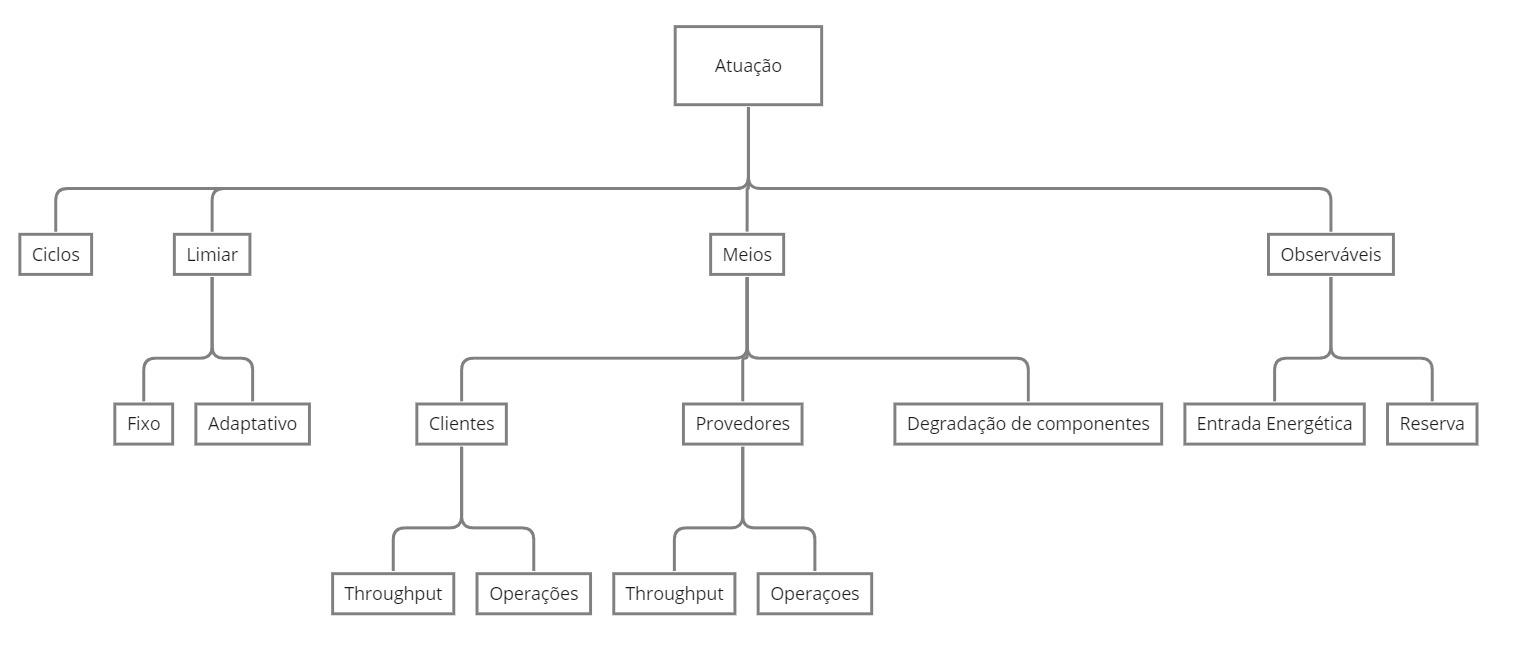
\includegraphics[width=1\textwidth]{Imagens/cap4/cap4taxonomia_throttling_atuacao.jpg}	
	
	Fonte: elaborado pelo autor.
\end{figure}

Em dispositivos \acs{IoT} orientados aos fatores energéticos, a atuação do padrão é dada ao monitorar a taxa de solicitações durante um espaço de tempo, esta janela temporal denomina-se Ciclo e esta disposito com categoria mais à esquerda no recorte disponivel na Figura \ref{fig:taxonomia_atuacao}. Durante um ciclo, clientes e provedores atuam realizando solicitações ou disponibilizando seus estados. Do ponto de vista da disponibilização dos recursos, durante um ciclo de carga, um dispositivo provedor configurado para tal, pode assumir abordagem de equidade entre os solicitantes ou algum critério de prioridade e privilégio. Em virtude disso, caso necessário um solicitante qualquer teria suas requisições atendidas enquanto acontece a negação do serviço para outro cliente com menor prioridade.

\textit{Throttling} utiliza mecanismos limitadores baseado em limiares, através da restrição no atendimento de solicitações. Uma vez definido limiar de atuação, a ação do limitador pode ser constante durante todo funcionamento do dispositivo, assim o mesmo valor limiar é aplicado independente de outros fatores durante todo o tempo, outra possibilidade é definir vários limiares que agem de maneira adaptativa de acordo com os modos de operação mapeados, tão logo determinado cenário seja alcançado, o dispositivo pode ajustar seu limiar de atuação para conservar seus recursos visando manter-se funcional. O comportamento do limiar de atuação passa pela analise cuidadosa da natureza das operações esperadas para o dispositivo e possui influencia sobre como o dispositivo irá se comportar. Quanto aos limiares, são classificados  como:

\begin{itemize}
    \item Limiar constante: Seu valor é fixado e estabelecido enquanto o dispositivo é projetado. Este limiar pode ser determinado considerando fatores como testes de desempenho, características do ambiente onde será inserido e requisitos operacionais. Todavia, uma vez definido, o limiar permanecerá constante ao longo de todo o momento em que  atividades são realizadas.
    
    Por exemplo, considere um dispositivo com uma dada capacidade de processar mensagens, este pode estabelecer um limiar constante para o máximo de requisições processáveis simultaneamente. Sendo assim, em toda operação, caso esse limiar de requisições seja atingido, irá ativamente rejeitar ou atrasar o atendimento das solicitações de serviço até que o valor de requisições retorne ao nível aceitado. 
    
    Esta abordagem, é bastante útil caso se conheça bem as capacidades do dispositivo e não se espera uma grande variação nas condições de operação ao longo do tempo. Embora oferte equidade do ponto de vista dos solicitantes, que tem suas requisições atendidas segundo os mesmos critérios independente do estado do dispositivo provedor, não é garantido que uso dos recursos será adequado caso ocorra mudanças repentinas ou flutuações significativas nos termos de funcionamento deste provedor.
    
    \item Limiar adaptável: Nesta abordagem, o comportamento do dispositivo é ajustado dinamicamente, por isso pode assumir um comportamento mais adequado ao observar suas condições de funcionamento através do monitoramento ou análise dos seus recursos. Permitindo atender as solicitações dos clientes, com performance adequada aos termos de operação que se encontre. Por exemplo, dado um sistema de segurança que geralmente possui dispositivos equipados com câmeras. Este provedor, deve enviar imagens capturadas por seus sensores para algum solicitante, seja uma central que passivamente recebe as gravações ou outra forma de demandante devidamente conhecido. Seja uma mudança observada em seus termos de funcionamento, o dispositivo poderá ter faixas de limiares distintas adequando-se ao estado encontrado, por exemplo, operações diurnas ou noturnas, conservando-se e garantido seu funcionamento dentro do acordo de serviço estabelecido.   
    
\end{itemize}

O dispositivo com limiar(es) de atuação, indica para o mecanismo \textit{throttling} em qual momento irá ser acionado, sendo capaz de adequar o modo de operação do dispositivo, depreciando seus serviços como mudança de comportamento, seja para interromper operações conforme Figura \ref{fig:cap2throttlingexample} ou reduzir sua taxa da transmissão. Com isso, aumentando seu tempo de inatividade e assim mitigando riscos enquanto se encontra em um modo restrito. 

Uma vez que os recursos energéticos observáveis se restabeleçam, pode-se assumir um comportamento de uso acentuado mediantes solicitações e a capacidade do dispositivo utilizar mais recursos disponíveis, incentivado pelo novo valor estipulado para o limiar de consumo. Esta capacidade de adaptação, permite que dispositivos mantenham algum equilíbrio enquanto conservam recursos e buscam performance, sustentado pela adaptação promovida pelos modos de operação definidos, garantindo assim suas disponibilidade nos termos das condições operacionais.


Qualquer aspecto que impacte ou influencie na capacidade do dispositivo em manter-se disponível deve ser considerado em sua atuação. Estes, ditos elementos observáveis, compreendem os componentes aos quais cabem a analise de estado, pois justificam a ação do mecanismo \textit{throttling}, que deverá indicar o comportamento do dispositivo para mante-lo adequado buscando evitar seu esgotamento energético. Para tal, se apresentam como os garantidores das condições energéticas do dispositivo: sua condição de entrada através da coleta de fonte energética e a capacidade de armazenamento dessa energia coletada em eventual \textit{buffer}. 

%\subsubsection{Meios}
%\label{cap4:atuacao_meios}
O comportamento de um dispositivo pode ser ajustado de acordo com suas circunstâncias. Diferentes meios são usados no processo de construção do mecanismo \textit{throttling} participante na adequação do comportamento à depender das características de atuação e a intenção ao limitar operações. Em detrimento disso, cabe observar papel à desempenhar pelo dispositivo pois, cada um deles apresentam em suas particularidades indicações sobre como agente limitador deverá atuar. Sendo assim, compõe os meios utilizados pelo agente limitador:

\begin{itemize}
	\item Meio 1: Da limitação sobre dispositivos clientes; 
	\item Meio 2: Da limitação sobre atividades do dispositivos provedor;
	\item Meio 3: Aspectos da degradação intencional de componentes demandantes.
\end{itemize}

Configura-se o Meio 1 a utilização dos mecanismos de throttling operam em referencia da  capacidade dos clientes em relação de sua taxa de vazão (\textit{throughput}) ou sobre a criticidade de suas operações. Sobre a taxa de vazão, é esperado que o limitador aplicado atue sobre a taxa de recebimento das mensagens em acordo com a capacidade do cliente para lidar com tais eventos. Sendo assim, o dispositivo cliente poderá limitar o envio de novas solicitações ou a sua disponibilidade para recebimento de novas informações de acordo com o modo de operação encontrado em decorrência das capacidades observadas que o colocam em tal modo.

Entende-se por criticidade para um cliente, o atributo que indica a importância das operações realizadas por este dispositivo em detrimento das consequências obtidas pela não realização de uma operação dita critica no cenário de atuação do dispositivo. Assim, é previsto dois cenários: um primeiro onde todas as operações tem igual importância, e um segundo, onde existam operações classificadas como criticas. Assim, de acordo com o segundo cenário, justifica-se que tais operações possam encontrar um modo com limiar de \textit{throttling} aliviado e por isso, cabe observar e definir tais valores para que caso ocorram operações privilégiadas, exista também a justificativa de maior tolerância quanto ao uso de recursos para o cumprimento destas. 

Certamente, para que seja possível um maior gasto de recursos pelas operações criticas, cabe também à fase concepção do dispositivo definir suas regras de compensação onde caso necessário, o dispositivo pode limitar outras operações, motivados a preservar parte do seus recursos que em outro momento seria utilizado por estas demandas menos privilegiadas.

Meio 2 compreende o controle de atuação no dispositivo provedor. De acordo com o seu estado durante um ciclo os mecanismos de throttling poderão atuar em conformidade aos recursos encontrados. Para tal, as estratégias de aplicação e definição de limiares passam pela observação da capacidade de vazão das múltiplas solicitações dos clientes, bem como da criticidade das operações realizadas. 

A taxa de vazão do um dispositivo provedor, é definida pela sua capacidade em atender demandas dos diversos solicitantes durante um ciclo, seja por limitação de transmissão (\textit{throughput}), por sua capacidade computacional em realizar tais operações ou mesmo seu modo de operação definidos em relação aos observáveis. Sendo assim, o mecanismo de throttling presente no provedor poderá se valer dos limiares estipulados através da análise dos recursos para operação e, em similaridade aos dispositivos clientes. A partir daí, caso o cenário encontrado seja apropriado, limitar o atendimento as solicitações de solicitantes considerados excessivamente demandantes ou não privilégiados.  

O limiar de atendimento de operações poderá suportar um sistema hierárquico, similar ao já definido sobre a criticidade das operações dos dispositivos clientes. Neste caso, é de conhecimento do dispositivo provedor quais solicitações são privilégiadas pois suas operações devem ser realizadas mesmo em um cenário mais restrito.

Quanto a observação das operações realizadas pelo dispositivo provedor, estas tem seu grau de criticidade atrelada a importância de tal operação na conjuntura ao que se destina o dispositivo. É importante destacar que a definição de limiares sempre busca garantir que o dispositivo não consuma seus recursos desnecessariamente, considerado um gasto excessivo. O Limiar de atuação deve ser revisto idealmente para atuar a todo momento que o panorama encontrado pelo dispositivo mude, seja pelo fim de um ciclo de atividades ou a medida que solicitantes sejam atendidos. Com isso, dado limiar deverá atuar protegendo o dispositivo provedor no decorrer de sua mudança de estado ao passo que realiza as operações. 

Pode-se ainda, anexar ao conjunto relacionado aos fatores utilizados para definição do limiar das operações, os aspectos ligados a degradação ativa nos componentes envolvidos nas operações  ou apenas de uso interno do dispositivo. Ao limitar alguma operação, apresenta-se a oportunidade para que o \textit{throttling} no dispositivo também possa restringir o uso de recurso energético de algum componente inativo, neste caso, encerra-se parcial ou totalmente a utilização energética dos componentes envolvidos com tais operações limitadas. 

Compreendendo os mecanismos dispostos no Meio 3, encontra-se a capacidade do nó em reduzir o consumo energético de algum componente embarcado mediante o cenário de escassez energética. Esta é uma manobra conhecida, diversos dispositivos submetem-se a esta manobra objetivando a conservação de seus recursos energéticos durante ciclos, especialmente quando não existe uma previsibilidade de uma nova oferta energética. Por exemplo, os aparelhos móveis adotam tal comportamento para que, quando um determinado valor energético em \textit{Storage} seja atingido, limitar ativamente os componentes menos críticos, por exemplo câmeras de alta definição ou alto-falantes, assim, o recurso energético usado por tais componentes podem ser conservados e disponibilizados para manter outros componentes dito essenciais até que o cenário de escassez se resolva. 

A entrada energética descrita na Subseção \ref{Capacidade de Coleta}, indica a capacidade do dispositivo em captar recursos energéticos através de mecanismo de coleta, uma vez que um dispositivo receba esta entrada, dará inicio um ciclo que por sua vez durará até a próxima oferta energética. Sobre a capacidade de armazenar energia, como decorrido na Subseção \ref{Capacidade de Armazenamento} é o indicativo do potencial que sua sua reserva energética (\textit{Storage}) pode chegar, para que em momento adequado, os valores armazenados sejam disponibilizados para suprir a demanda energética operacional.

A capacidade do dispositivo em entender a dinâmica dos fatores que interagem com os valores coletados na forma de entrada energética através do seu \textit{Power Supply} e reserva (\textit{Storage}) são fundamentais para garantir maior disponibilidade. Estes fatores compreende os observáveis, grupo motivador do ajuste de comportamento dos mecanismos providos pela atuação do \textit{throttling}. 


\subsection{Motivadores}

Além das operações realizadas, a implementação do padrão throttling passa por avaliar os agentes que impactam diretamente o comportamento do dispositivo. Este, também deve considerar a atuação do mesmo enquanto dispositivo \acs{IoT}. 

Desta forma, a mudança de comportamento do dispositivo motiva-se em: tão logo os fatores de tomada de decisão forem alcançados, adequar-se para que estes fatores agora considerados divergentes, sejam superados motivados pela mudança de modo de operação buscando retornar ao cenário que representa as capacidades de atendimento do dispositivo.   Por isso, o agente limitador deve agir de maneira suficientemente rápida para que a mudança de estados seja alcançada o mais brevemente possível, referente à capacidade do dispositivo em dispender recursos para realizar operações. 

No trabalho \cite{zhang_toward_2018}, equipamentos capazes de observar seus recursos energéticos, atuam modificando seu comportamento para preservar energia enquanto permanecem na expectativa de uma entrada energética prevista. Sendo assim, a motivação de aplicação do agente limitante é preservar alguma condição energética, prolongando a disponibilidade dos componentes ditos críticos. Portanto, a motivação dos dispositivos em limitar seu comportamento passa pela análise do estado dos recursos observáveis e a intenção que se deseja alcançar em acordo com agente limitante. Por sua vez em, \cite{gong_sleep_2022} aborda a capacidade de decidir se os dispositivos devem hibernar, realizar operações ou transmitir seus resultados. Estas operações são realizadas motivadas pela analise dos recursos energéticos de maneira que dado um cenário o dispositivo permaneça inativo por mais tempo, ou realize mais medições.

No contexto de computação dirigida à energia, em quaisquer cenário que o dispositivo se encontrar, caso um limiar de atuação seja atingido a alteração de comportamento precisa ocorrer de modo adequado, mitigando, com isso, perdas desnecessárias ou não previstas, causadas por ajuste inapropriados de comportamento. Considerando que o ajuste demorado potencialmente coloca o dispositivo em não ter um modo de operação adequando às suas condições reais.

Para justificar a atuação dos mecanismos de limitação, é preciso definir quais são seus  motivadores, estes carregam o propósito declarado para restringir operações em concordância com a causa motivadora. Assim, é de interesse da observação das capacidades energéticas, ajustar o comportamento do dispositivo motivado do que pretende-se obter através disso, os motivadores para uso de \textit{throttling} sob essas circunstancias são:

\begin{enumerate}
	\item Preservar recursos energéticos. 
	Evitar gasto excessivo ou inadequado é primeiro motivador de um agente limitante embarcado em dispositivos com restrições energéticas, pretende-se com isso manter o dispositivo operando adequadamente em relação das capacidades energéticas e com isso dispendendo recursos de maneira sustentada ao passo que a energia coletada durante os ciclos anteriores seja suficiente para todas operações realizadas, enquanto preserva seus recursos presentes.
	
	\item Restabelecimento da condição energética.
	Quanto a recuperar seus recursos energéticos, entende-se que o dispositivo poderá através da analise de seus observáveis, adotar comportamento limitado motivado pela expectativa de restabelecer seus recursos energéticos a patamar acima do encontrado em \textit{storage}. Neste caso, pretende-se manter-se em modo de operação que favoreça dispender menos recurso possível durante os próximos ciclos até que seus recursos observáveis retornem aos valores desejados. Uma vez alcançado um estado desejado, o dispositivo poderá reavaliar seu comportamento e ajustar-se para o modo de operação considerado adequado. 
\end{enumerate}

\begin{comment}
	
estão dispostos em cenário de disponibilidade energética previsível onde é necessário em prever a quantidade futura de energia coletável disponível para recarga. O problema foi apresentado na forma de um \ac{MDP} onde os dispositivos podem adequar seu comportamento de acordo com expectativa energética vindoura para recarga. 


acima do que de fato deveriam Ocasionando até mesmo, um cenário de maior esgotamento energético do que previso

coloque o agente em um modo de operação inadequado, fora do esperado. A depender de como as operações ocorrem, o modo de operação terá capacidade de criar um cenário de esgotamento energético acelerado, em outra parte, a limitação inapropriada poderá causar sobrecarga de atividades para outros elementos da rede, por exemplo.
	

Estes aspecto podem ter seus valores pré-estabelecidos, porém é comum enfrentar situações onde os valores tidos como justificadores de um comportamento não sejam suficientemente adequados, seja por uma falha na previsibilidade de um recurso ou evento não tolerável. Por exemplo, é relativamente comum um cenário onde dispositivos que exploram energia solar diurnalmente enfrentem alguma escassez energética motivados por eventos climáticos não previstos. Com isso, colocam em risco sua disponibilidade, pois caso seja mantido o comportamento dito adequado e previamente estabelecido podem levar o dispositivo a um alterações em sua disponibilidade não previstas ou perdas em performance. 

No contexto de dispositivos com capacidade de coleta energética, fatores pré-estabelecidos são comumente encontrados, ciclos de recarga na forma de capacidade de coleta, a capacidade de armazenamento do dispositivo e a sazonalidade da fonte energética coletável. O conjunto dos valores  desses fatores presentes no dispositivo, indicam o estado energético deste agente. Dado um estado energético esperado, pode-se previamente definir como o dispositivo se comportará. Mesmo assim, também vale ressaltar que estes elementos energéticos estão relacionados às variações e toda sorte de situações que o dispositivo provedor enfrenta enquanto agente em campo. Diversos esforços foram realizados para melhorar a maneira como um agente observa seu estado energético e define seu comportamento, mas para que seja possível adequar-se concretamente à estes fatores encontrados, o agente deve ter a capacidade de analisar as operações e o cenário onde se encontra, tanto individualmente quanto, se possível, em conjunto com outros elementos colaboradores. Assim, é possível realizar ajustes prontamente nos limiares de atuação, tão logo perceba-se que os valores estimados previamente e o seu estado esperado divirjam causando comportamento fora do desejado.

\end{comment}  









